\newcommand{\CoreModDesc}[1]{\subsection{#1}\index{Core Modules!#1}}
\newcommand{\CoreMod}[1]{\code{#1}}

\chapter{Core-modules Reference}
In this chapter I will describe all core (\module{pyDCPU}) modules.
A core module implements a new feature (protocol,device,...) to the
PPLT system. This is the atomic element of the PPLT devices and servers.

A core module is always a small python script with a specific interface 
zipped into an archive. This archive have to consists of at least two
files. One named \texttt{meta.xml} containing the meta-info of the
core-module. The second file have to be named \texttt{\_\_init\_\_.py}.
This file should include or contain the python source-code of the core
module.

In the following sections I will describe all core modules available until
now. Or all that I know of.



\section{Master modules}
Master modules are modules that are used in the PPLT devices. So this
modules implement the features to access a device, like the interface,
bus protocol, device commands, ...



%\CoreModDesc{Master.Interface.SendMail}
%This module implements the sending of e-mails via a
%specified SMTP host. \note{You have to have the permission 
%to send a e-mail of this host.} 



\CoreModDesc{Master.Interface.Socket}
This modules implements the basic TCP socket support for the PPLT system. 
With this module you can connect to other hosts over any tcp/ip based network
(Internet). This is used in the PPLT device \textit{PLC.FP-WEB} to connect to 
the tunneled ToolPort of a Panasoinc PLC. This module is able to hanle 
multible connections, so you don't need to load a 
\CoreMod{Master.Interface.Socket}-module for each connection you want.

\subsubsection{Parameters}
This module needs only one parameter:
\begin{tableiii}{l|p{10cm}|l}{textrm}{Parameter}{Description}{Default value}
\lineiii{TimeOut}
        {This parameter specifies the read-timeout for the socket 
         connection(s) in seconds. This should be a string with a floating 
         point number in it like '0.5' for a timeout of an half second.}
        {'0.0'}
\end{tableiii}

\subsubsection{Addresses}
This module need a address, thats specifies the host and port of the TCP 
connection. So if you connect to this module with an address "10.1.1.1:100"
a connection to the host "10.1.1.1" at the port 100 will be opend. See 
example for more details. \notice{If the connection to the host fails
the first time, it will be retryed each time you read/write from/to the 
module until the connection can be etablished.} 

\subsubsection{Example}
\begin{figure}[ht]
    \label{fig:coremod02}
    \centering
    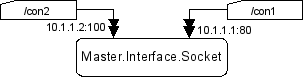
\includegraphics[scale=1]{coremod02.png}
    \caption{This figure shows the module-map of the socket-example.}
\end{figure}    
This example opens two connection to different hosts and ports:
\lstinputlisting{coremod02.py}



%
% Serial interface module:
%
\CoreModDesc{Master.Interface.UniSerial}
The \CoreMod{Master.Interface.UniSerial} core module implements the serial
interface for the PPLT system. This module needs the Python library 
\code{pySerial}. You can get this library from the URL 
\url{http://serial.sourceforge.net}. 

The settings of this module can be changed at runtime by symbols connected to
the addresses \emph{speed}, \emph{parity} \emph{timeout}.

\subsubsection{Parameters}
This module 4 parameters to setup. 
\begin{tableiii}{l|p{10cm}|l}{textrm}{Parameter}{Description}{Default value}
\lineiii{Port}
        {This is the number of the serial interface, the moudle should use. 0 
         means \code{ttyS0} or \code{COM1}, 1 means \code{ttyS1} etc. This
         parameter is not optional!}
        {---}
\lineiii{Speed}        
        {This is the speed in Baud the serial interface will be set to. This
         parameter is not optional!} 
        {---}
\lineiii{Parity}
        {This parameter specifies the parity check (settings) of the serial 
         inteface. 'Odd', 'Even', 'None' are valid values. This parameter
         is optional.}
        {'None'}
\lineiii{TimeOut}
        {This parameter sets the timeout for reading from the serial 
         interface in seconds. All floatingpoint numbers are valid an
         \code{None} means blocking-read.}
        {\code{None}}
\end{tableiii}
\notice{Some parameters can be reset at runtime by symbols connected to this 
module at special addresses. See next paragraph for details.}

\subsubsection{Addresses}
\begin{tableiii}{l|l|p{10cm}}{testrm}{Address}{Type}{Description}
\lineiii{---}
        {\code{TStream}}
        {This is the \emph{data-channel} to the serial-interface. Meaning 
         reading from this will read from the serial interface and writeing
         into a connection to this will write into the serial-interface.}
\lineiii{speed}
        {\code{TInteger}}
        {By this connector you'll be able to change the settings of the serial
         interface at runtime. Write an integer to a connection to this address
         will (try) to reset the baudrate to the value. See example for details.}
\lineiii{parity}
        {\code{TString}}
        {Writing strings like 'even', 'odd' or 'none' into this connector, will
         reset the setting of the serial interface. Reading from the connector
         will infrom you about the current setting.}
\lineiii{timeout}
        {\code{TFloat}}
        {Writing to this connector will reset the timeout for reading from 
         the serial interface.}
\end{tableiii}

\subsubsection{Example}
\begin{figure}[ht]
    \label{fig:coremod01}
    \centering
    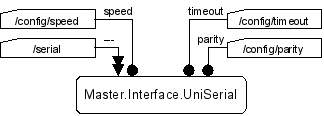
\includegraphics{coremod01.png}
    \caption{This figure shows the module-map of the UniSerial-example.}
\end{figure}    
This example shows how to setup the \CoreMod{UniSerial} and how to change the 
settings at runtime:
\lstinputlisting{coremod01.py}








%\CoreModDesc{Master.Interface.WGet}




%
% Transport layer of the Mewtocol:
%
\CoreModDesc{Master.Transport.MEWCOM-TL}
This module implements the transport-layer of the MEWTOCOL. The MEWTOCOL 
normally doesn't distinguish between the tansport and command layer. So
this module is only usfull in combination with the \CoreMod{MEWCOM-CL}
core-module that implements the command messages of the MEWTOCOL.

\subsubsection{Parameters}
This module needs only one parameter that specifies if a cecksum should
be calculated and adde to the MEWTOCOL message. By defualt this parameter
is set to \code{"True"}

\begin{tableiii}{l|p{10cm}|l}{textrm}{Parameter}{Description}{Default}
\lineiii{BCC}
        {This parameter specifies if a bcc (checksum) should be claculated
         for each packet send. This parameter doesn't contol the if the
         checksum of a recived packet will be checked. This will allways be 
         done (if the packet contains a checksum)\footnote{The MEWTOCOL 
         protocol allows that a packet doesn't contain a checksum. In this 
         case the checksum 'XX' will be set to indicate that the checksum
         should not be checked.}.  
        }{'True'}
\end{tableiii}       

\subsubsection{Addresses}
Each module or symbol have to set a address for the connection to this 
module. This address specifies the address of the destination the 
MEWTOCOL messages are send to. 
\begin{tableiii}{l|l|p{10cm}}{textrm}{Address}{Type}{Description}
\lineiii{0..255}
        {\code{TSequence}}
        {This address specifies the destination of the messages send.}
\end{tableiii}

\subsubsection{Example}
Because of this module is not usefull alone, please look at the example for 
the \CoreMod{MEWCOM-CL} core module.



%
% PPI module:
%
\CoreModDesc{Master.Transport.PPI}
This Core-Module implements the PPI protocol. It can be used to access the Siemens
SIMATIC S7 series PLCs. In this state of developing this module can't assable an
dispatch fragmentated packages. But in the most cases this is not needed. 

\subsubsection{Parameters}
This module needs only one parameter:
\begin{tableiii}{l|p{10cm}|l}{textrm}{Parameter}{Description}{Default}
\lineiii{Address}
        {This parameter specifies the PPI address of the PC. This is in the 
         most cases 0. But you have to set a value for this parameter!}
        {}
\end{tableiii}

\subsubsection{Addresses}
If you connect other modules or symbols to this module you'll need to specify
an address. This address is a number between 0 and 255. 
\begin{tableiii}{l|l|p{10cm}}{textrm}{Address}{Type}{Description}
\lineiii{0-255}{\code{Sequence}}
        {This address specifies the address of the device in the PPI BUS. 
         Writeing into the connection will cause a packet send to the device
         addressed by this address. Also reading from the connection will only
         return the content addressd to the setted Parameter \var{Address} and
         from the device addressd by this address.}
\end{tableiii}

\subsubsection{Example}
\begin{figure}[ht]
    \label{fig:coremod07}
    \centering
    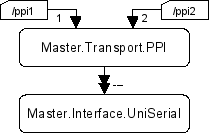
\includegraphics{coremod07.png}
    \caption{This figure shows the module-map of the PPI-example.}
\end{figure}    
This example shows how to tunnel the PPI bus by the symbol tree. For an more
usefull example please look the the Example for the \CoreMod{S7} core-module.
\lstinputlisting{coremod07.py}



%
% ReadLine module.
%
\CoreModDesc{Master.Transport.ReadLine}
This module can be used if you want to do some line-orientated communication.

This is often used for simple protocols for the serial interface. For example
the AT commands for modems but also the Mewtocol by Panasonic (FP0 and FP1) 
uses a line-orientated protocol to send or recive commands to/from the PLC.  

So this module have to be used as a child of a module that provides
\code{TStream} or \code{TSequence} connections.

\subsubsection{Parameters}
This module needs a parameter to specify the \emph{line-end} character(s).
\begin{tableiii}{l|p{10cm}|l}{textrm}{Paramter}{Description}{Default}
\lineiii{LineEnd}
        {A hex-encoded string that the module will use as a sign for the 
         line-end. And also all data send over this module will be extended
         with this string.}
        {0A0D} 
\end{tableiii}

\subsubsection{Addresses}
This module knows only one address: no address.
\begin{tableiii}{l|l|p{10cm}}{textrm}{Address}{Type}{Description}
\lineiii{---}
        {\code{TSequence}}
        {All data written into this connector will be extended by the set 
         line-end. And also if you read from this connector it will block 
         until the set line-end character(s) appear in the data-stream.
         \textbf{Note:} The whole line will be then returned!}
\end{tableiii}

\subsubsection{Example}
\begin{figure}[ht]
    \label{fig:coremod10}
    \centering
    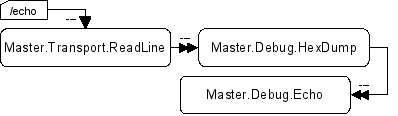
\includegraphics{coremod10.png}
    \caption{This figure shows the module-map of the ReadLine-example.}
\end{figure}    
This example shows on the one hand the usage of the \CoreMod{ReadLine} module.
On the other hand it is a quite good test for the \CoreMod{Echo} module. 
This example write a string into \CoreMod{ReadLine} that extends the string 
with the line-end. Then it will send this message to the \CoreMod{Echo} module.
Then it trys to read from \CoreMod{ReadLine} that trys to read a complete 
line from his parent (\CoreMod{Echo}) strips the line-end characters and
return the string. If all goes well the same string will be returned. To see
what's going on a \CoreMod{HexDump} module will be plugged between the 
\CoreMod{Echo} and \CoreMod{ReadLine} modules.
\lstinputlisting{coremod10.py}



%
% Agilent 5462x series oscilloscopes 
%
\CoreModDesc{Master.Device.5462X}
This module implements the command messages to access an Agilent 
oscilloscopes. This module only supports the message format used 
by the serial interface of the oscilloscope. So you need to connect
this module (indirect) to the \CoreMod{Master.Interface.UniSerial}
core-module.

\subsubsection{Parameters}
This module need two parameters to be set up. These parameters specify the
primary and secondary signal source. If you only want to use the primary
source you should set the secondary to the same source like the primary.
\begin{tableiii}{l|p{10cm}|l}{textrm}{Parameter}{Description}{Default}
\lineiii{PSource}
        {This specifies the primary source. This can be one of A0 (analog \#1),
         A1 (analog \#2), M (math) or F (form).}{---}
\lineiii{SSource}
        {This specifies the secondaray source. Look at \var{PSource} for more
         details}{---}
\end{tableiii}         
\bf{To be continued} \bf{To be continued}

%
% Panasonic A200 Imagechecker
%
%\CoreModDesc{Master.Device.A200}



%
% GSM compatible mobile-phone.
%
\CoreModDesc{Master.Device.GSM}
With this device you can send SMS or read status information about a GSM 
compatible mobile-phone. You only need to append this device on a serial
interface (IrDA, bluetouth may also work).

\subsubsection{Parameters}
This module needs no parameters.

\subsubsection{Addresses}
\begin{tableiii}{l|l|p{10cm}}{textrm}{Address}{Type}{Description}
\lineiii{network}{\code{TInteger}}
        {If you read from this connection you'll get the network-state of
         the mobile phone.}
\lineiii{battery}{\code{TInteger}}
        {If you read from this connection you'll get the battary-level of
         the mobile-phone in percent.}
\lineiii{quality}{\code{TInterger}}
        {If you read from this connection you'll get the signal-quality of
         the connection to the access-point the mobile-phone is dialed in.}
\lineiii{errorrate}{\code{TInteger}}
        {If you read from this connection you'll get the errorrate of the
         connetion to the access-point the mobile-phone is dialed in.}
\lineiii{manufacturer}{\code{TString}}
        {Returns the name of the manufacturer.}
\lineiii{model}{\code{TString}}
        {Returns the modelname.}
\lineiii{sms:NUMBER}{\code{TString}}
        {If you write into this connection, you'll send a sms to the given 
         number! For example \code{sms:0123456789}.}
\end{tableiii}

\subsubsection{Example}
In this example I will show how to read the information form the mobile-phone 
and to send this data as a short \emph{Report-SMS}.
\lstinputlisting{coremod12.py}

%
% Command-messages for the Panasonic FP0 and FP1
%
\CoreModDesc{Master.Device.MEWCOM-CL}
This core-module implements the command messages of the MEWTOCOL. This 
protocol is used to access the Panasonic FP0 FP2 PLCs. So you can access
the markers of these PLCs using the \CoreMod{Master.Transport.MEWCOM-TL},
\CoreMod{Master.Device.MEWCOM-CL} core-modules and a interface module like 
\CoreMod{Master.Interface.UniSerial} or \CoreMod{Master.Interface.Socket}.

\subsubsection{Parameters}
This module needs no parameters to be set up.

\subsubsection{Addresses}
You have to set a address to connect a symbol to this module! With this 
address you specify the marker you want to get/set. Additional there is a
address called \code{"STATUS"} that controls the state of the PLC 
(\emph{run}/\emph{stop}).
\begin{tableiii}{l|p{2cm}|p{10cm}}{textrm}{Address}{Type}{Description}
\lineiii{STATUS}
        {\code{TBool}}
        {By this address you can control the state of the PLC. If it is 
         \code{True} then the PLC is in the \emph{Run} mode. You can also
         get the state of the PLC by reading this value.}
\lineiii{\emph{Marker}}
        {\code{TBool} or
         \code{TInteger}}
        {By setting a marker-address as the address for the connection to this 
         module, you are able to access (read/write) this marker. So the type 
         of the connection you'll get depends on the marker-address you set.} 
\end{tableiii}

\subsubsection{Example}
\begin{figure}[ht]
    \label{fig:coremod11}
    \centering
    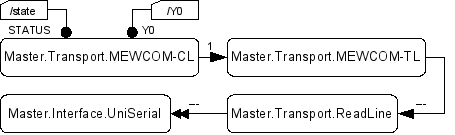
\includegraphics{coremod11.png}
    \caption{This figure shows the module-map of the MEWCOM-CL example.}
\end{figure}    
This example shows how to access a FPx using the \emph{ToolPort} (serial interface).

\lstinputlisting{coremod11.py}



%
% Command messages for the Siemens SIMATIC S7-200 (may be other)
%
\CoreModDesc{Master.Device.S7}
This module implements the command-messages of the Siemens SIMATIC S7(-200). 
With this module and the \CoreMod{Master.Transport.PPI} and 
\CoreMod{Master.Interface.UniSerial} it is possible to access the S7 over the 
PPI bus. To do this you must configure the serial interface in a special way. 
Look at the example to find out how. This module can generate messages that 
cause the S7 to send the value of the requested marker. To specify the marker 
you want to get you have to connect a symbol with this module with the name of
the marker as address. It could be possible that not all availabe marker can be
read. If you know some of them please let me know.

\subsubsection{Parameters}
This module needs no parameters to be set up.

\subsubsection{Addresses}
The address you have to specify to connect a symbol to this module should be 
the name of the marker you want to get/set.
\begin{tableiii}{l|p{2cm}|p{10cm}}{textrm}{Address}{Type}{Description}
\lineiii{\emph{Marker}}
        {\code{TBool}, \code{TInteger}}
        {With the address you specify the marker you'll access. So the type 
         of the values you'll get depends on the marker you'll set. So if you 
         access an boolean marker you'll get values typed \code{TBool} if you
         access byte,word and double word Markers you'll get values types
         \code{TInteger}.}
\end{tableiii}

\subsubsection{Example}
\begin{figure}[ht]
    \label{fig:coremod08}
    \centering
    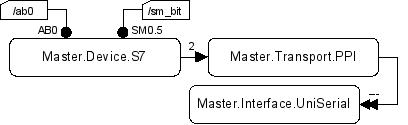
\includegraphics{coremod08.png}
    \caption{This figure shows the module-map of the S7-example.}
\end{figure}    
In this example I'll access (read/write) the markers SM0.5 (special marker 0 bit 5) and AB0
(output byte 0).

\lstinputlisting{coremod08.py}



%
% ECHO module
%
\CoreModDesc{Master.Debug.Echo}
This module echoes all data writte to it at reading from it. It can be used to
debug other modules. This is a so called \emph{root}-module. It can't be 
loaded as a child of an other module!

\subsubsection{Parameters}
This module needs no parameters!

\subsubsection{Addresses}
This module has only one addresses: no address.
\begin{tableiii}{l|l|p{10cm}}{textrm}{Address}{Type}{Description}
\lineiii{---}
        {\code{TStream}}
        {If you write into a symbol connected to this module, the data will be
         buffered and the next time you read from it the buffer (or a part of 
         it) will be returned.}
\end{tableiii}

\subsubsection{Example}
\begin{figure}[ht]
    \label{coremod06}
    \centering
    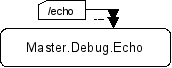
\includegraphics{coremod06.png}
    \caption{This figure shows the module-map of the Echo-example.}
\end{figure}    
This is a simple echo-example... ... the classic.

\lstinputlisting{coremod06.py}



%
% HexDump Module 
%
\CoreModDesc{Master.Debug.HexDump}
This module is a simple trafic dumper. It dumps all data going throught it
into the logging-system with loglevel \emph{debug}. So you can read it from
your logfile or \code{stderr}. Simply plug this module between two modules
to record all trafic.

\subsubsection{Parameters}
This module needs no parameters!

\subsubsection{Addresses}
This module has only one address: no address! 
\begin{tableiii}{l|p{2cm}|p{10cm}}{textrm}{Address}{Type}{Description}
\lineiii{---}
        {\code{TStream} or \code{TSequence}}
        {All data written to this module will be written to the parent and 
         read vica versa. So the type of the connection will depend on the
         type of the parent-connection.}
\end{tableiii}

\subsubsection{Example}
\begin{figure}[ht]
    \label{fig:coremod05.py}
    \centering
    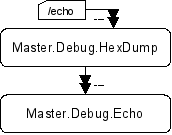
\includegraphics{coremod05.png}
    \caption{This figure shows the module-map of the HexDump-example.}
\end{figure}    
This module uses the echo module to show how the trafic in read and write 
direction will be dumped:
\lstinputlisting{coremod05.py}



%
% Null module (the black hole)
%
\CoreModDesc{Master.Debug.Null}
This is a very simple module, that works like the /dev/null device file on 
Linux. If you read from this module, you'll get a string with zero-bits and
if you write into this module nothing will happens. This module swallow all
you write into it.

\subsubsection{Parameters}
This module needs no parameters to be set up.

\subsubsection{Addresses}
This module has only one valid address: no address.
\begin{tableiii}{l|l|p{10cm}}{textrm}{Address}{Type}{Description}
\lineiii{---}
        {\code{TStream}}
        {This will be the connection to the \CoreMod{Null} module. Id you
         write into this connection the module will swallow all data and
         nothing will happen. If you read from this module you'll get a 
         stream of zero-bits.}
\end{tableiii}

\subsubsection{Example}
\begin{figure}[ht]
    \label{fig:coremod09}
    \centering
    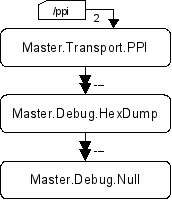
\includegraphics{coremod09.png}
    \caption{This figure shows the module-map of the Null-Example.}
\end{figure}    
This example shows a configuration to debug a non \emph{root} module. In this 
case it is the \CoreMod{Master.Transport.PPI} core-module. To get some 
information about the packages the PPI module sends the core-module 
\CoreMod{Master.Debug.HexDump} is used.  \notice{This example raises an 
exception, because the PPI module expect a correct answer from the 
\emph{virtual} device (in this case the core-module 
\CoreMod{Master.Debug.Null}).
\lstinputlisting{coremod09.py}



%
% Random-generator module
%
\CoreModDesc{Master.Debug.Random}
This module implements a random-generator, that can generate data for every 
symbol-type supported by the \module{pyDCPU}. So this module can be used to 
test almost all facilities of the system. 

\subsubsection{Parameters}
This module needs no parameters. 

\subsubsection{Addresses}
\begin{tableiii}{l|l|p{10cm}}{testrm}{Address}{Type}{Description}
\lineiii{Bool}
        {\code{TBool}}
        {Provide a random boolean value.}
\lineiii{Integer}
        {\code{TInteger}}
        {Provide a random integer value between 0 and 100.}
\lineiii{Float}
        {\code{TFloat}}
        {Provide a random floating point number between 0 and 1.}
\lineiii{String}
        {\code{TString}}
        {Provide a random string of a random length between 1 and 79 containg 
         printable characters.}
\lineiii{ArrayBool}
        {\code{TArrayOfBool}}
        {The name tells everything. The length of the array is randomly 
         between 1 and 3.}
\lineiii{ArrayInteger}
        {\code{TArrayOfInteger}}
        {Array of integer of random length between 1 and 3.}
\lineiii{ArrayFloat}
        {\code{TArrayOfFloat}}
        {Array of floating point numbers with variable length between 1 and 
         3.}
\lineiii{ArrayString}
        {\code{TArrayOfString}}
        {Array of string with variable length (of array) between 1 and 3.}
\lineiii{Stream}
        {\code{TStream}}
        {Provides an random data string. The data are printable character.
         The number of bytes returned is less than equeal the number you 
         wanted to read. To read from a symbol connected to this address,
         please use the method \method{SymbolTreeRead().}}
\lineiii{Sequence}
        {\code{TSequence}}
        {A sequence of random data. The data contains only printable 
         characters and the length varies between 1 and 79.}
\end{tableiii}

\subsubsection{Example}
This is a simple example that uses all types:
\lstinputlisting{coremod03.py}



%
% Statistic module
%
\CoreModDesc{Master.Debug.Statistic}
This module collects statistical values of the data flowing through it. You 
can use this module to improve or debug your own modules or even to observe
the PPLT system. This module is quite easy to use: simply plug this between 
two other modules and you are able to observe the trafic between them.
\notice{You can only observe modules that provides a \code{TStream} or 
\code {TSequence} connection.}

\subsubsection{Parameters}
This module needs no parameters!

\subsubsection{Addresses}
There are several addresses provideing the statistical data. If you use no 
address to connect to this module a \code{TStream} or \code{TSequence} 
connection to the parent will be returned. This connection to the parent will
be used to collect the statistical data. 

\begin{tableiii}{l|p{2cm}|p{10cm}}{textrm}{Address}{Type}{Description}
\lineiii{---}
        {\code{TStream} or \code{TSequence}}
        {This is the data-tunnel to the parent of the 
         \CoreMod{Statistic}-module. The type of the connection depends on
         the type of the connection to the parent module. You see, it is only
         possible to connect the \CoreMod{Statistic}-module to a parent that
         provides a \code{TStream} or \code{TSequence} connection.}
\lineiii{read\_data}
        {\code{TInteger}}
        {Returns the number of bytes read from the parent.}
\lineiii{write\_data}
        {\code{TInteger}}
        {Returns the number of bytes written to the parent.}
\lineiii{read\_speed}
        {\code{TFloat}}
        {Returns the number of bytes per second read from parent since 
         module-loading. This value is the average of the whole time since
         module-loading.}
\lineiii{write\_speed}
        {\code{TFloat}}
        {Returns the number of bytes written to the parent since the module 
        was loaded. This value is the average of the whole time.}
\lineiii{error}
        {\code{TInteger}}
        {Returns the number of read/write-errors since the module was loaded.
         This must not be an indicatior for bugs in the parent modules because
         also timeouts will be recorded.}
\end{tableiii}

\subsubsection{Example}
In this example the serial interface will be exported by the symbol tree.
The \CoreMod{Statistic}-module records the trafic throught the serial 
interface.
\lstinputlisting{coremod04.py}



\section{Export modules}
Export or better server-modules are used to export the symbols stored in the 
symbol-tree to other applications like visualisations etc. You can start a
server by calling the \code{ExporterAdd()} method. You can stop the server
by calling the \code{ExporterDel()} method with the id of the server 
(returned by the \code{ExporterAdd()} method). 

Servers are running in there own thread, so the main application doesn't block
if you're starting a new server. 

Some of the servers don't know any authentication, but the PPLT system needs 
to know who access the symbol tree. So each server can be started with a 
\emph{default-user}. If the server doesn't use authentication, the server 
will run with the rights of the given defaut user. \notice{So be carefull
with this default user and allways take a user, that has the lowest rights.}

Also you can define a \emph{server-root} on loading. By this you can export 
only a part (only the folder you've specified as the server-root) of the
symbol-tree by the specific server. Look at the core library refrerence for
details.


\CoreModDesc{Export.JVisu}
This server-module implements a \emph{JVisu} socket-server for the open
sourec Java visualiation. This server knows no authentication so be
carefull with the default-user.

\subsubsection{parameters}
This module needs only two parameters to be set up. The address the server
will be bind to and the TCP port the server will listen on for new 
connections.
\begin{tableiii}{l|p{10cm}|l}{textrm}{Parameter}{Description}{Default}
\lineiii{Address}
        {This parameter specifies the address the server will bind to.}
        {---}
\lineiii{Port}
        {This parameter specifies the port the server will listen for new
         connections.}
        {---}
\end{tableiii}



\CoreModDesc{Export.SimpleExport}
This module implement a simple XML-RPC server that serves some functions to 
access the symbols and folders on the exported symbol-tree. This server 
provides some functions to authenticate but if the authentication was missed,
the default user will be used. So please be carefull with the default-user 
you'll define. 

XML-RPC is a system and language independent protocoll to call 
remote-procedures so your applications can access the symbol-tree independent
from the language you use or the system your application will run on.

\subsubsection{Parameters}
This module needs two parameters to be set up. The address the server will be
bind to and the TCP port the server will listen to.
\begin{tableiii}{l|p{10cm}|l}{textrm}{Parameter}{Description}{Default}
\lineiii{Address}
        {This parameter defines the address the server will be bind to.}
        {---}
\lineiii{Port}
        {This parameters specifies the TCP port the server will listen for 
         new connections.}
        {---}
\end{tableiii}

\subsubsection{Exported methods}
The \code{logon()} method can be used to start a session. This method takes 
two arguments. The first argument is a string and contains the username and
the second is a string containing the password. The method will return a 
string with the sessionid or \code{false} on error. The returned sessionid
can be used as an argument for all other methods to authenticate your calls.
If you miss the session-argument, you calls will be executed with the rights
of the defualt-user specified at the loading of the server.

The \code{logoff()} method quits a session. The method will need the sessionid
you've got from the \code{logon()} method as argument.

The \code{get()} method can be used to get the value from the given symbol. 
So the method will take a string argument containing the full path to the 
symbol. 

The \code{set()} method will set the value of the given symbol to the given
value. So this method will take at least two arguments. The first is a string
containing the full path to the symbol and the second is the value. This method
will return true on success and false on error.

The \code{listfolders()} method will return a array containing all folders 
in the given folder. So the first argument should be a string containing the
full path to the folder (for all root-folders use '/') the content you want to
get. The returned array will be an array of strings with all folder-names. If
there are no folders the method will return an empty array.

The \code{listsymbols()} method works like the \code{listfolders()} method. It
returns all symbols in the given folder. So the first argument should be a 
string containing the full path to the folder you want to list.



\CoreModDesc{Export.PPLTWeb}
This coremodule implements a simple web-server to serve the symbol-tree. You 
can access the symbol-tree and the values of the stored symbols by a simple 
web-browser. This server known a basic http-authentication, so you the 
\emph{default user} will be ignored.

\subsubsection{Parameters}
This server-module will need two parameters to be set up. The address the 
server will be bind to and the TCP port the server will listen on for new
connections.
\begin{tableiii}{l|p{10cm}|l}{textrm}{Parameter}{Description}{Default}
\lineiii{Address}
        {This parameter defines the address the server will be bind to.}
        {---}
\lineiii{Port}
        {This parameters specifies the TCP port the server will listen for 
         new connections.}
        {---}
\end{tableiii}


